\documentclass[border=0mm]{standalone}
\usepackage{tikz}
\usepackage{amsmath}
\usepackage{amsmath}
\usetikzlibrary{calc, angles, quotes}
\begin{document}
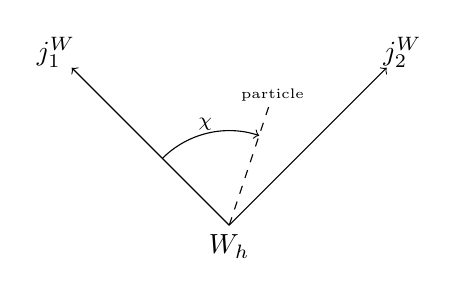
\begin{tikzpicture}
  \coordinate(O) at (0.0, 0.0);
  \coordinate(a1) at (-2.0, 2.0);
  \coordinate(p) at (0.5, 1.5);
  \coordinate(a2) at (2.0, 2.0);
  \draw[->] (O) -- (a1) node[pos=1.1] {$j^{W}_{1}$};
  \draw[->] (O) -- (a2) node[pos=1.1] {$j^{W}_{2}$};
  \draw[dashed] (O)-- (p) node [pos = 1.1] {\tiny particle};
  \draw[<-] pic [draw, angle radius=1.2cm, angle eccentricity=1.1,"$\chi$" font=\scriptsize] {angle=p--O--a1};
  \draw (O) node [below]{$W_{h}$};

\end{tikzpicture}
\end{document}
